\chapter{Algoritmo de Grover}
%El algoritmo de Grover es un AC que encuentra con alta probabilidad la entrada única de una función de caja negra que produce un valor particular de salida, usando tan sólo $O(\sqrt{N})$ evaluaciones de la función, donde $N$ es el tamaño del dominio de la función. El análogo clásico de este algoritmo requiere $O(N)$ evaluaciones de la función, pues, el elemento correcto podría ser el $N$-ésimo en ser evaluado y se deben evaluar uno por uno. La aplicación directa de este algoritmo es como algoritmo de búsqueda en una base de datos. Sin embargo, su aplicación más eficiente es como subrutina en diversos procesos de optimización.

El algoritmo de Grover es un AC que realiza una búsqueda en una secuencia no ordenada de datos con $N=2^n$ entradas. Clásicamente esta búsqueda tendría un orden de complejidad de $O(N)$, pues, como los datos no están ordenados, la cantidad promedio de evaluaciones que se deben realizar crece linealmente con la cantidad de entradas. En el caso del algoritmo de Grover, la complejidad de la búsqueda es de $O(\sqrt{N})$, pues se requieren aproximadamente $\frac{\pi\sqrt{N}}{4}$ iteraciones para hallar la entrada deseada. En cuanto a la cantidad de qubits requeridos, se necesitan $O(\log_2 N)$ qubits, pues se debe realizar un estado superpuesto donde cada componente de la superposición represente una entrada de la secuencia de datos.

Supongamos que la secuencia de datos ordenada tiene la siguiente función asociada:

\begin{equation}
    f(x) =
    \begin{cases}
        1 & \text{si } x = \omega \\
        0 & \text{si } x \neq \omega
    \end{cases}
\end{equation}

Donde $\omega$ es el dato que se desea encontrar. Esta función devuelve 1 si se evalua la entrada que almacena el dato deseado y 0 en cualquier otro caso.

El algoritmo de Grover se basa en la disponibilidad de un operador cuántico, llamado \textit{oráculo}, tal que se introduzca un fase global de $\pi$ si $f(x_0)=1$ y deje el estado del sistema intacto si $f(x_0)=0$. Es decir, el oráculo realiza una reflexión alrededor de $\ket{\omega}$.

\begin{equation}
    U_\omega \ket{x} = (-1)^{f(x)} \ket{x} =
    \begin{cases}
        \ket{x} & \text{si } x \neq \omega \\
        - \ket{x} & \text{si } x = \omega
    \end{cases}
\end{equation}

\begin{equation}
U_\omega = \mathds{1} - 2 \ketbra{\omega}{\omega}
\end{equation}

Además de éste, se necesita otro operador de reflexión, $U_s$, el cual realiza una reflexión alrededor del estado de superposición uniforme $\ket{s} = \frac{1}{\sqrt{N}} \sum\limits_{x=0}^{N-1} \ket{x}$. Así, por el hecho de la geometría plana elemental de que el producto de dos reflexiones es una rotación, se logra aproximar el estado del sistema al estado asociado a la entrada deseada.

\begin{equation}
U_s = 2 \ketbra{s}{s} - \mathds{1}
\end{equation}

Veamos lo que sucede al aplicar esta secuencia de rotaciones sobre el estado $\ket{s}$:

\begin{align*}
    U_\omega \ket{s}
    &= (\mathds{1} - 2 \ketbra{\omega}{\omega}) \ket{s} \\
    &= \ket{s} - 2 \ketbra{\omega}{\omega} \ket{s} \\
    &= \ket{s} - \frac{2}{\sqrt{N}} \ketbra{\omega}{\omega} \sum\limits_{x=0}^{N-1} \ket{x} \\
    &= \ket{s} - \frac{2}{\sqrt{N}} \ket{\omega}
\end{align*}

\begin{align*}
    U_s (\ket{s} - \frac{2}{\sqrt{N}} \ket{\omega})
    &= (2 \ketbra{s}{s} - \mathds{1}) (\ket{s} - \frac{2}{\sqrt{N}} \ket{\omega}) \\
    &= 2 (\ket{s} - \frac{4}{N} \ket{s}) - (\ket{s} - \frac{2}{\sqrt{N}} \ket{\omega}) \\
    &= \ket{s} - \frac{4}{N} \ket{s} + \frac{2}{\sqrt{N}} \ket{\omega} \\
    &= \frac{N-4}{N} \ket{s} + \frac{2}{\sqrt{N}} \ket{\omega}
\end{align*}

Ahora veamos lo que sucede al aplicar esta secuencia de rotaciones sobre el estado $\ket{\omega}$:

\begin{align*}
    U_\omega \ket{\omega}
    &= (\mathds{1} - 2 \ketbra{\omega}{\omega} \ket{\omega} \\
    &= \ket{\omega} - 2 \ket{\omega} \\
    &= - \ket{\omega}
\end{align*}

\begin{align*}
    U_s (-\ket{\omega})
    &= (2 \ketbra{s}{s} - \mathds{1}) (-\ket{\omega}) \\
    &= -\frac{2}{\sqrt{N}} \ket{s} + \ket{\omega} \\
\end{align*}

Se observa que al aplicar $U_s U_\omega$ sobre $\ket{s}$, se amplifica la componente de $\ket{\omega}$ en la superposición de $\frac{1}{\sqrt{N}}$ a $\frac{3N-4}{N \sqrt{N}}$. Es decir que la probabilidad de medir el valor deseado crece de $\frac{1}{N}$ a $9 (1-\frac{4}{3N}) \frac{1}{N}$.

\begin{align*}
    \bra{\omega} U_s U_\omega \ket{s}
    &= \frac{N-4}{N} \frac{1}{\sqrt{N}} + \frac{2}{\sqrt{N}} \\
    &= \frac{3N-4}{N \sqrt{N}}
\end{align*}

\begin{align*}
    \abs{\bra{\omega} U_s U_\omega \ket{s}}^2
    &= \frac{(3N-4)^2}{N^3} \\
    &= 9 (1-\frac{4}{3N}) \frac{1}{N}
\end{align*}

Por otro lado, se observa que al aplicar $U_s U_\omega$ sobre $\ket{\omega}$, aparece una componente de $\ket{s}$, así que en ese caso, la probabilidad de medir el valor deseado disminuye. Por lo que debe existir una cantidad de iteraciones $k_{max}$ tras las cuales se alcanza la probabilidad máxima de medir $\ket{\omega}$, partiendo de $\ket{s}$ y a partir de donde esta probabilidad empieza a disminuir.

De esta manera, el algoritmo de Grover consiste en aplicar $k_{max}$ veces $U_s U_\omega$, partiendo del estado $\ket{s}$, es decir rotar este estado hasta que se aproxime lo más posible a $\ket{\omega}$.

\begin{figure}[H]
\[ \Qcircuit @C=1.4em @R=1.8em {
\lstick{\ket{0}} & {/^n} \qw & \gate{H^{\otimes n}} & \gate{U_{\omega}} & \gate{U_s} & \meter & \cw \\
& & & \rstick{\hspace{-13pt} k_{max} \text{ veces}}
\gategroup{1}{4}{1}{5}{1.5em}{_\}}
} \]
\caption{Circuito del algoritmo de Grover, $k_{max}$ desconocido.}
\end{figure}

Para hallar $k_{max}$, veamos el ángulo que se rota con cada aplicación de $U_s U_\omega$. Primero definamos el estado $\ket{s^\prime}$ como la superposición uniforme de todos los estados de la base computacional excepto $\ket{\omega}$, es decir:

\begin{align}
    \ket{s^\prime} &= \frac{1}{N-1} \sum\limits_{x \neq \omega} \ket{x} \\
               &= \frac{\sqrt{N}}{\sqrt{N-1}}\ket{s} - \frac{1}{\sqrt{N-1}} \ket{\omega}
\end{align}

Los estados $\ket{s^\prime}$ y $\ket{\omega}$ son ortonormales, $\braket{s^\prime}{\omega} = 0$, por lo que generan un espacio bidimensional de Hilbert. Este espacio contiene a $\ket{s}$, pues:

\begin{equation}
    \ket{s} = \frac{\sqrt{N-1}}{\sqrt{N}}\ket{s^\prime} + \frac{1}{\sqrt{N}}\ket{\omega}
\end{equation}

Además, se ha visto que $U_s U_\omega \ket{s}$ y $U_s U_\omega \ket{\omega}$ se escriben en función de sólo $\ket{s}$ y $\ket{\omega}$. Así que podemos inducir que $(U_s U_\omega)^k \ket{s}$ pertenece al espacio generado por $\{\ket{s^\prime}, \ket{\omega}\}$, donde $k \in \{0, 1, 2, ...\}$. Esto indica que este espacio contiene al plano en el que se realizan las rotaciones $U_s U_\omega$.

Ahora que conocemos una base del plano de rotación, podemos hayar el ángulo que se rota con cada aplicación de $U_s U_\omega$.

\begin{align*}
    U_\omega \ket{\psi}
    &= (\mathds{1} - 2 \ketbra{\omega}{\omega}) (\alpha \ket{s^\prime} + \beta \ket{\omega}) \\
    &= \alpha \ket{s^\prime} - \beta \ket{\omega}
\end{align*}

\begin{align*}
    U_s (\alpha \ket{s^\prime} - \beta \ket{\omega})
    &= (2 \ketbra{s}{s} - \mathds{1}) (\alpha \ket{s^\prime} - \beta \ket{\omega}) \\
    &= \alpha \left(2 \frac{\sqrt{N-1}}{\sqrt{N}} \ket{s} - \ket{s^\prime}\right) - \beta \left(\frac{2}{\sqrt{N}} \ket{s} - \ket{\omega}\right) \\
    &= \alpha \left((2\frac{N-1}{N} - 1) \ket{s^\prime} + 2\frac{\sqrt{N-1}}{N}\ket{\omega}\right) \\
    &\qquad - \beta \left(\frac{2\sqrt{N-1}}{N}\ket{s^\prime} + (\frac{2}{N}-1)\ket{\omega}\right) \\
    &= (\alpha \frac{N-2}{N} - \beta \frac{2\sqrt{N-1}}{N}) \ket{s^\prime} \\
    &\qquad + (\alpha\ 2\frac{\sqrt{N-1}}{N} + \beta  \frac{N-2}{N}) \ket{\omega} \\
\end{align*}

De aquí se deduce que $\cos(\Delta\theta) = \frac{N-2}{N}$ y que $\sin(\Delta\theta) = 2\frac{\sqrt{N-1}}{N}$. De hecho, se comprueba que:

\begin{equation*}
    \cos^2(\Delta\theta)+\sin^2(\Delta\theta)
    = \frac{(N-2)^2}{N^2} + 4\frac{N-1}{N^2}
    = \frac{N^2-4N+4}{N^2} + 4\frac{N-1}{N^2}
    = 1
\end{equation*}

Ahora escribimos las componentes de $\ket{s}$ en función del ángulo inicial $\theta_0$:

\begin{align}
    \cos(\theta_0) &= \frac{\sqrt{N-1}}{\sqrt{N}} \\
    \sin(\theta_0) &= \frac{1}{\sqrt{N}}
\end{align}

Finalmente, lo que se quiere es que:

\begin{equation}
    \theta_0 + k \Delta\theta \to \frac{\pi}{2}
\end{equation}

Es decir, que:

\begin{align}
    \cos^{-1}(\frac{\sqrt{N-1}}{\sqrt{N}}) + k\cos^{-1}(\frac{N-2}{N}) &\to \frac{\pi}{2} \\
    \sin^{-1}(\frac{1}{\sqrt{N}}) + k\sin^{-1}(2\frac{\sqrt{N-1}}{N}) &\to \frac{\pi}{2}
\end{align}

Si tomamos $N \gg 1$ en (4.12), tenemos que:

\begin{align}
    2k \frac{1}{\sqrt{N}} &\to \frac{\pi}{2} \\
    k_{max} &\approx \frac{\pi \sqrt{N}}{4}
\end{align}

\begin{figure}[H]
\centering \includegraphics[width=0.3\linewidth]{img/grover_geometry.png}
\caption{Interpretación geométrica del operador difusión}
\end{figure}

\section{El algoritmo}

\begin{figure}[H]
\[ \Qcircuit @C=1.4em @R=1.8em {
\lstick{\ket{0}} & {/^n} \qw & \gate{H^{\otimes n}} & \gate{U_{\omega}} & \gate{U_s} & \meter & \cw \\
& & & \rstick{\hspace{-13pt} \lfloor\frac{\pi \sqrt{N}}{4}\rfloor \text{ veces}}
\gategroup{1}{4}{1}{5}{1.3em}{_\}}
} \]
\caption{Circuito del algoritmo de Grover.}
\end{figure}

\begin{enumerate}
    \item Preparar el estado fiducial.
    \item Aplicar la transformada de Walsh-Hadamard.
    \item Realizar la iteración de Grover $\lfloor \frac{\pi}{4} \sqrt{N} \rfloor$ veces.
    \begin{enumerate}
        \item Aplicar $U_{\omega}$.
        \item Aplicar $U_s$.
    \end{enumerate}
    \item Realizar la medida $\Omega$.
\end{enumerate}

\section{Simulación}

Se ha realizado una simulación del algoritmo de Grover en Wolfram Mathematica implementando $U_{\omega}$, $U_s$ y la transformada de Hadamard, directamente, de manera matricial, de acuerdo a las definiciones dadas anteriormente. Por otro lado, se ha realizado una simulación del algoritmo de Grover en Python definiendo todas las operaciones y transformaciones en base a sus construcciones circuitales, a partir de las compuertas nativas de los transmones, resolviendo la ecuación maestra del sistema al aplicar cada compuerta nativa. A la primera la llamaremos la simulación matemática, y a la segunda, simulación circuital. El código de ambas simulaciones se encuentra en el apédice (APENDICE).

En el caso de la simulación matemática, sólo se ha simulado el caso sin pérdidas. Sin embargo, en el caso de la simulación circuital, se ha simulado el sistema tanto sin pérdidas, como con pérdidas. En el caso del sistema con pérdidas, se ha utilizado la ecuación maestra de Lindblad con los operadores de colapso $\sigma_{-_i}$ y tasa de relajación $\gamma = 25KHz$. Primero compararemos las dos simulaciones sin pérdidas para analizar la precisión del solucionador de ecuaciones maestras.

En la figura (FIGURA) se puede observar la gráfica de la evolución de la probabilidad de medir cada estado en cada iteración. Como se puede observar, ambas figuras son bastante similares. Por otro lado, la fidelidad entre los estados finales de ambas simulaciones es <++>. Por lo que la precisión del solucionador de ecuaciones maestras causó un error correspondiente a una pérdida de <++> de fidelidad.

\begin{figure}[H]
    \centering
    \begin{subfigure}[m]{0.45\textwidth}
        \centering
        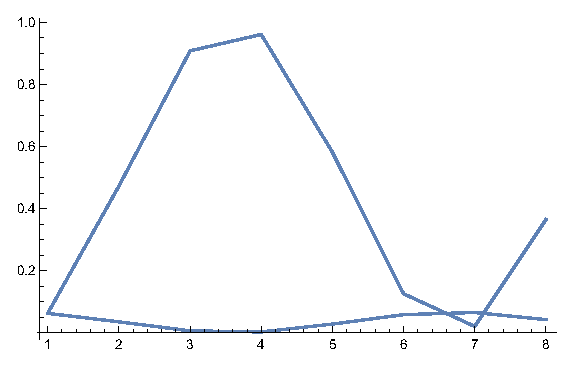
\includegraphics{img/Grover-2_gr1.eps}
        \caption{Rx}
    \end{subfigure}
    \begin{subfigure}[m]{0.45\textwidth}
        \centering
        \includegraphics[width=0.9\linewidth]{img/groveralllossless.png}
        \caption{Ry}
    \end{subfigure}
    \caption[]{Compuertas Rx, Ry y Rz en la esfera de Bloch}
    \label{fig:groverlosslesscomp}
\end{figure}

Ahora, compararemos los resultados de la simulación circuital con y sin pérdidas. Como se puede ver en la figura (FIGURA), en el caso con pérdidas, los estados que no contienen el valor deseado dejan de tener la misma probabilidad. Los estados que involucran el estado base ganan probabilidad debido a la relajación de los qubits. La fidelidad entre los estados resultantes de los casos con y sin pérdidas es de <++>.

Aunque la fidelidad sea tan baja, la probabilidad del estado deseado sigue siendo lo suficientemente alta como para obtener el resultado deseado x/x veces.

\begin{figure}[H]
    \centering
    \begin{subfigure}[m]{0.45\textwidth}
        \centering
        \includegraphics[width=0.9\linewidth]{img/groveralllossless.png}
        \caption{Ry}
    \end{subfigure}
    \begin{subfigure}[m]{0.45\textwidth}
        \centering
        \includegraphics[width=0.9\linewidth]{img/groverpairlossless.png}
        \caption{Rz}
    \end{subfigure}
    \caption[]{Compuertas Rx, Ry y Rz en la esfera de Bloch}
    \label{fig:groverlosscomp}
\end{figure}

